\section{UNSAT core refinement}
As all other MUS extractors, our algorithm cannot generate a minimal (irreducible) core in one shot.
To get a smaller core, we need to restart our tool with the current core we have. In this section several heuristics
are applied to our algorithm to increase the probability to generate a smaller core in next iteration.

\subsection{Leaf polynomial cancellation due to quotients}
First of all, before we start a new iteration of our GB engine, we can analyze the information we get from last 
iteration and remove redundancy.
In the last section we extract an UNSAT core by including all leaf polynomials in our tree to refutation "1".
The tree represents a linear combination with polynomial coefficients
of leaf polynomials. For example, in Fig.\ref{fig:tree} refutation "1" can be written as equation
$$1 = c\cdot f_2 + f_5 + {\bf \it f_3} + f_4 + f_1 + ac\cdot f_2 + a\cdot f_2 + {\bf \it f_3} + c\cdot f_2 + f_2$$
By combining like terms, the RHS polynomial can be simplified as
$$1 = f_1 + (ac+a+1)f_2 + f_4 + f_5$$
Note that polynomial $f_3$ is eliminated as $f_3+f_3 = 0 \pmod 2$. 
Thus $f_3$ is redundant in the core we previously extracted.

\subsection{Refining heuristics}
After eliminating all redundant polynomials, we can call our GB engine with the new core.
A effective heuristic should enhance the probability that the refutation "1" is composed by fewer polynomials.
In our GB computing algorithm, we use a strategy to pick critical pairs such that polynomials with 
larger indices get involved as late as possible:
$$(f_1,f_2)\to(f_1,f_3)\to(f_2,f_3)\to(f_1,f_4)\to(f_2,f_4)\to\cdots$$
Meanwhile, for the reduction process $Spoly(f_i,f_j)\xrightarrow{F}_+ f_{new}$, we pick divisor
polynomials from $F$ following the order of polynomial indices. Therefore, by renaming the polynomial indices
and moving specific polynomials to small indices, we can increase the likelihood they are selected into the UNSAT core.

A straightforward inspiration is, by moving polynomials that are most likely included in the 
refutation tree to small indices, we can reach a fixpoint with fewer calls to GB engine.
In this paper, we use 2 criteria to increase the probability that a polynomial is included in the 
refutation tree.  The one is the "distance" to refutation "1",
the other is the "frequency" a polynomial appears in refutation tree.

"Distance" in a refutation tree corresponds to the number of arcs on the shortest path from refutation "1"
to leaf polynomial
Usually polynomials with shorter distance to "1" are used as divisors in later steps of polynomial reductions,
which indicates they will more generally have lower degree leading terms. 
If we use a degree-lexicographic order, then term cancellations reduce the degree of the polynomial. So polynomials with lower degree leading terms are more 
likely to be used for reduction, such that the possibility they appear in refutation tree is larger. 
Similarly, the motivation for "frequency" of appearance is as follows:
polynomials appearing frequently in refutation tree also indicates they have some properties make
them "favourable" in UNSAT core selection. For example, their leading terms may contain a variable that suppose to be included in a necessary clause of a minimal core. 

Our tool applied both heuristics: we sort the polynomials in the core by "distance" criterion,
then use frequency as tiebreaker -- if there are multiple polynomials with same "distance", we put the one appears most frequently in last refutation tree first. 
We use an example to illustrate our heuristic.
\vspace{5mm}\\
{\it Example:}\ \ Consider a set of 6 polynomials which is UNSAT:
\begin{align*}
f_1 &: x_1x_3+x_3\\
f_2 &: x_2 + 1\\
f_3 &: x_2x_3+x_2\\
f_4 &: x_2x_3\\
f_5 &: x_2x_3 + x_2 + x_3 + 1\\
f_6 &: x_1x_2x_3 +x_1x_3
\end{align*}
After the first iteration, we get a tree of refutation in Fig.\ref{fig:refine}(a). 
\begin{figure}[hbt]
\centering
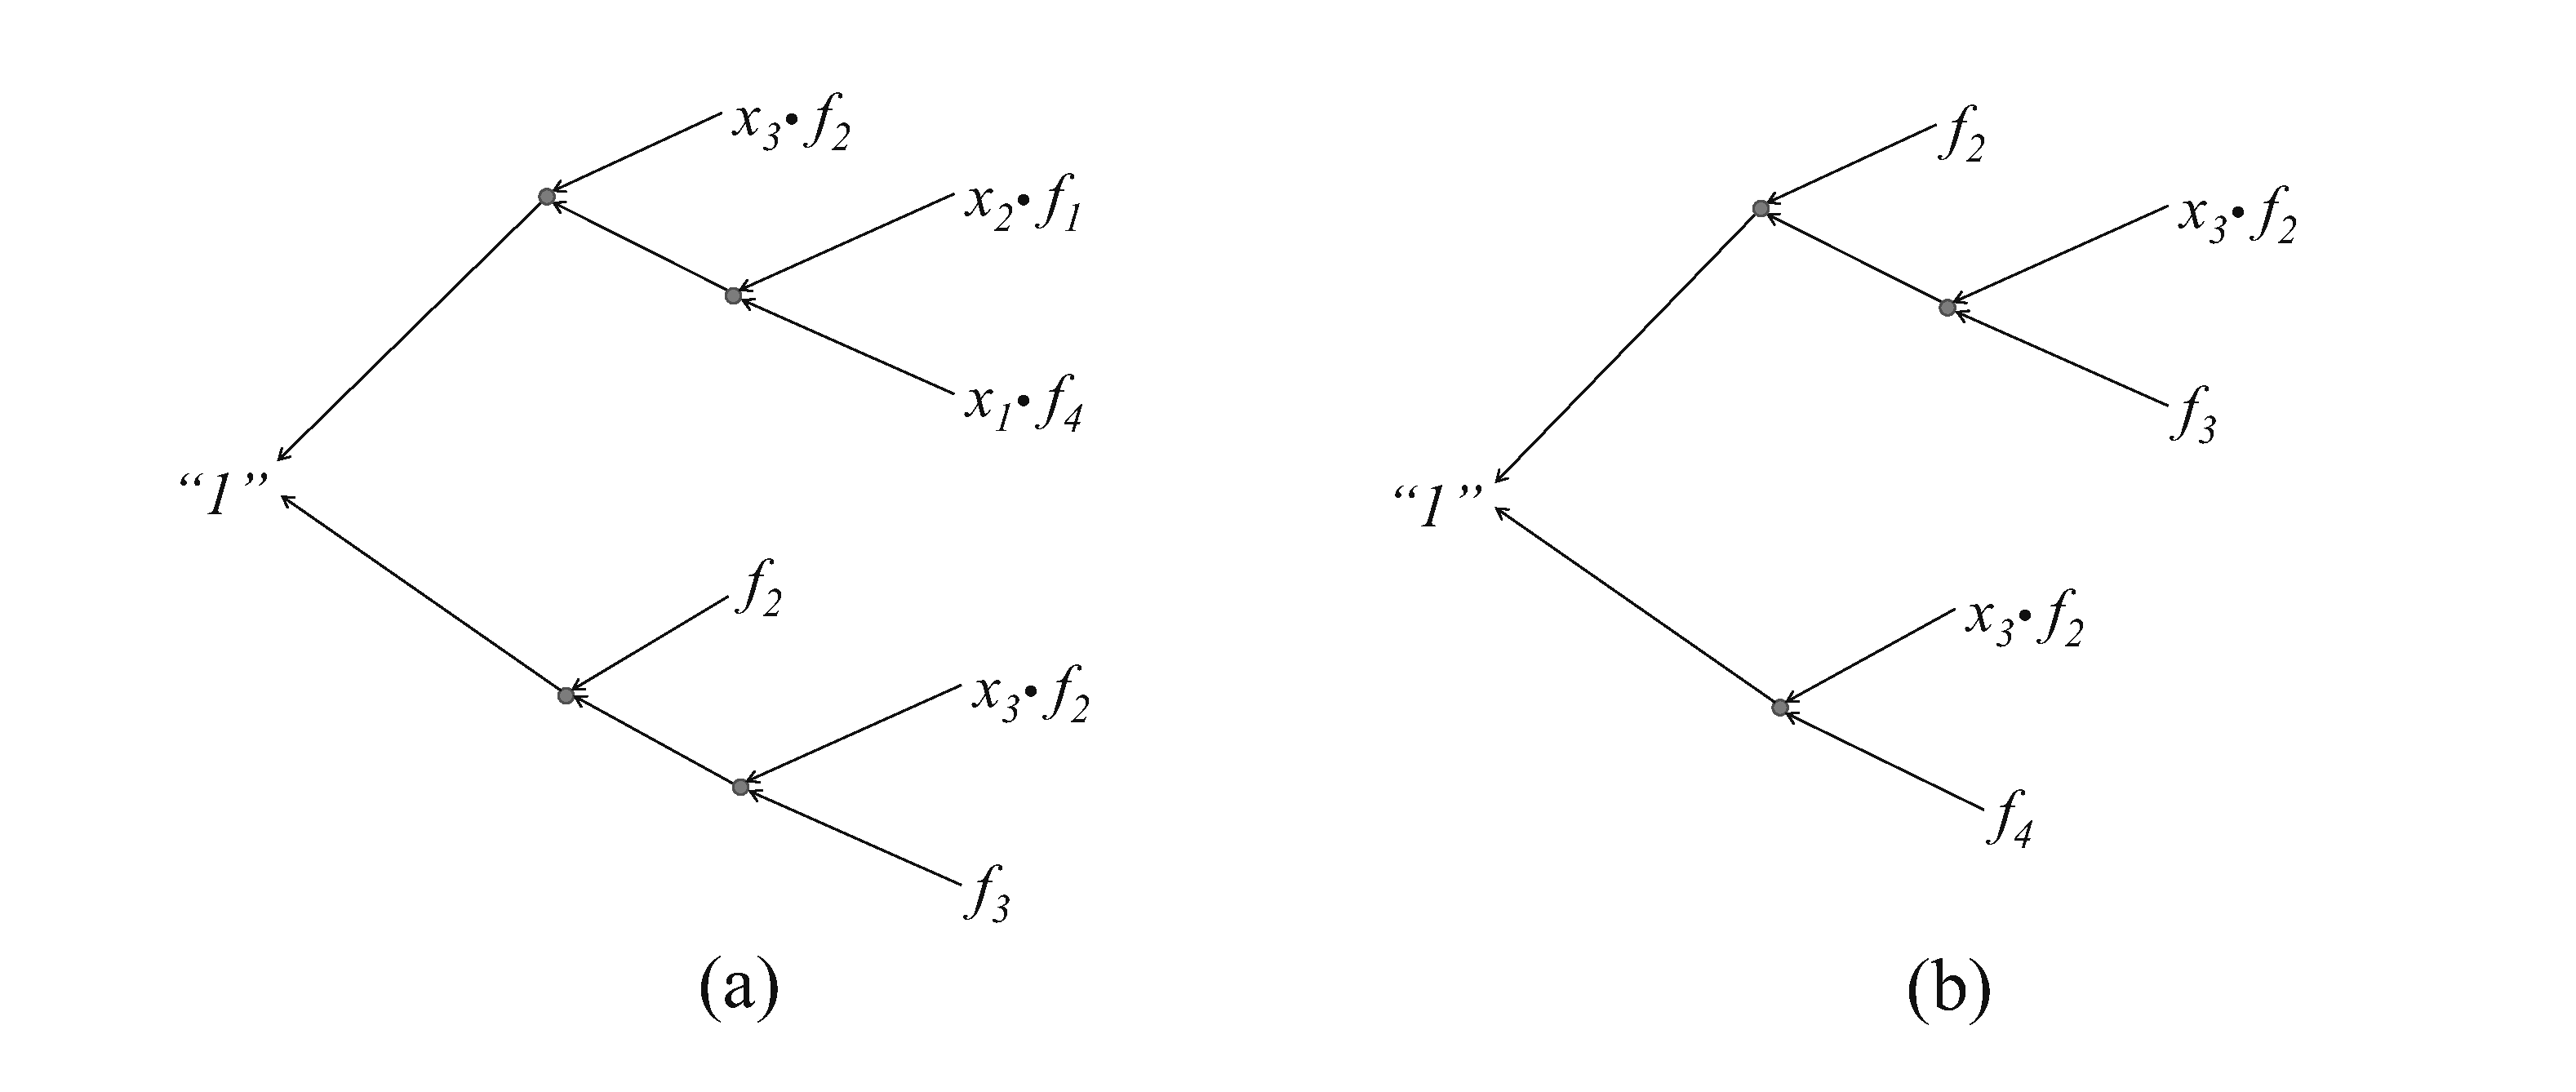
\includegraphics[scale=0.25]{core_refine.eps}
\caption{Refutation trees of core refinement example}
\label{fig:refine}
\end{figure}
"Distance" from $f_2$ to "1" is 2, so we put it in first place. The "distance" and "frequency" for other 
polynomials are identical, so we keep their ordering untouched. We re-index the polynomial set
$$f_1'=f_2, f_2' = f_1, f_3' = f_3, f_4' = f_4$$
and apply our GB-core algorithm on $\{f_1',f_2',f_3',f_4'\}$. The result is as
Fig.\ref{fig:refine}(b) shows. We reach a fixpoint, and the core $\{f_1', f_3', f_4'\}$ i.e. $\{f_2,f_3,f_4\}$ is proved to be minimal.